

%%%%%%%%%%%%%%Empieza la presentacion%%%%%%%%%%%%%%%%%%%%%%%%%%%%%%%%%%%%

%\begin{frame}
%\frametitle{Esquema}
 %   \tableofcontents
%\end{frame}


\begin{frame}\frametitle{Visi\'{o}n por computador}
  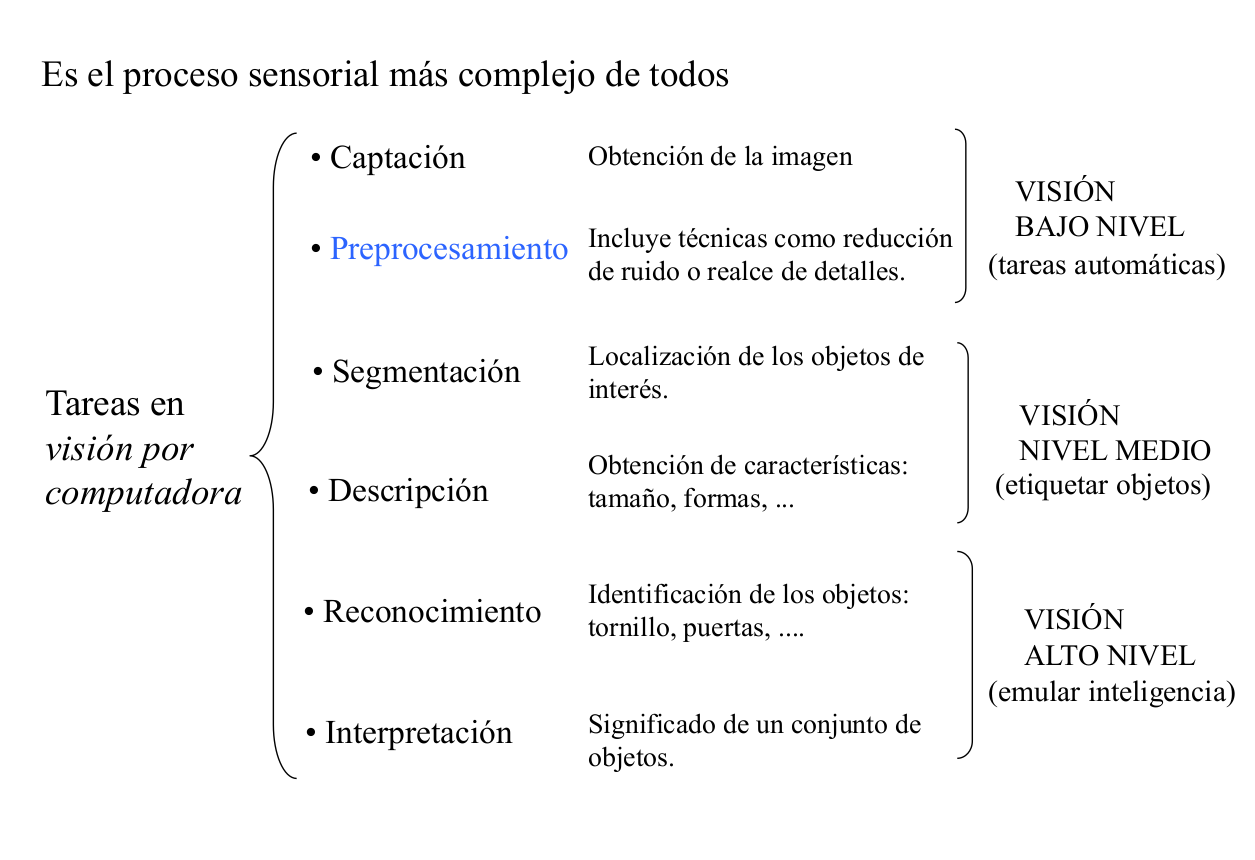
\includegraphics[width=10cm]{Figures/Clasificacion.png}
\end{frame}

\subsection{Adquisici\'{o}n y repesentaci\'{o}n de im\'{a}genes}

\begin{frame}
\frametitle{Adquisici\'{o}n de im\'{a}genes}
Las im\'{a}genes provienen de diferentes fuentes y se digitalizan  a trav\'{e}s de diferentes medios.
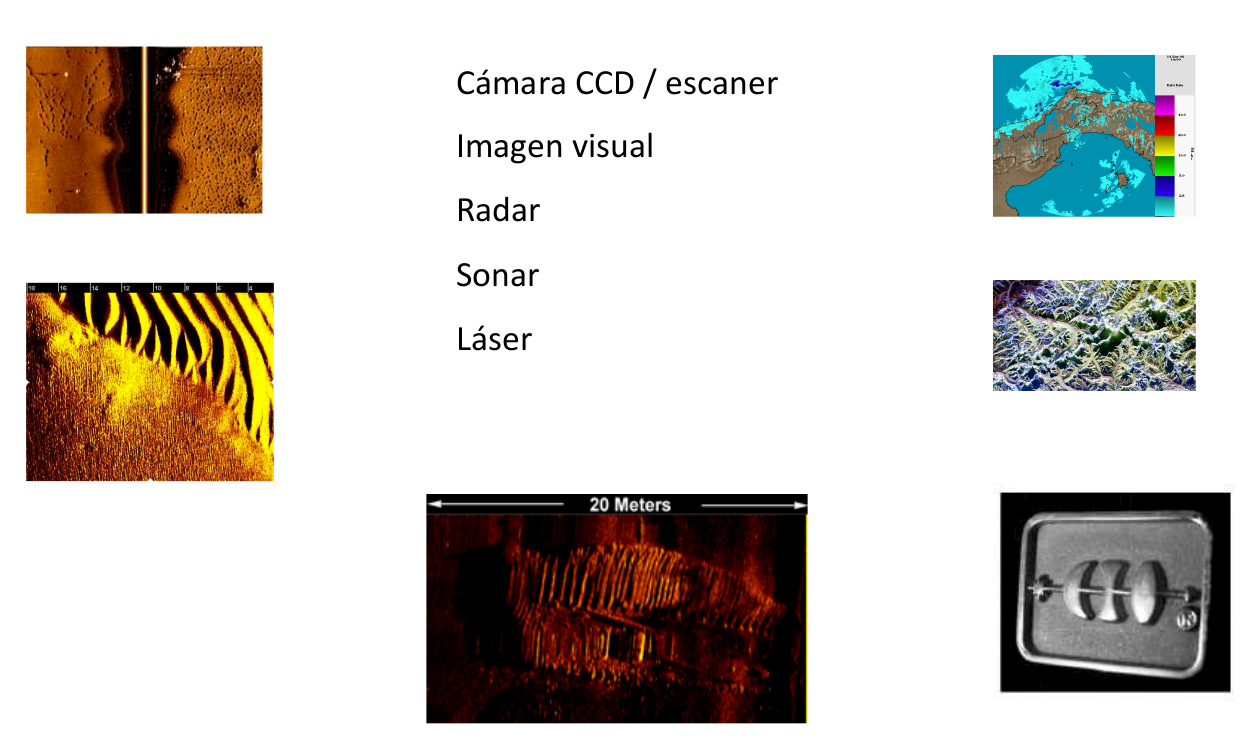
\includegraphics[width=10cm]{./Figures/AdquisicionImagenes}
\end{frame}

\begin{frame}
\frametitle{Representaci\'{o}n de im\'{a}genes en el computador}

\small

Una imagen es una se\~{n}al bidimensional (x,y) con uno o varios canales:

\vspace{-0.1cm}

\begin{itemize}

\small

\visible<2->{

\item \textbf{Imagen de intensidad (B/N) o de escala de grises}: en cada pixel (posici\'{o}n de la matriz de valores) se almacena un \'{u}nico valor que representa la intensidad luminosa en el punto correspondiente.

\vspace{-0.3cm}

\begin{columns}[t]
\hspace{1cm}\begin{column}{1.8cm}

\includegraphics[width=1.7cm,trim={0cm 0cm 0cm 0cm},clip,angle=0]{./Figures/Moon.eps}

\end{column}

\hspace{-0.5cm}\begin{column}{8cm}


\visible<3->{

\footnotesize
Es una matriz de MxN valores:

\vspace{-0.15cm}
\begin{itemize}

\scriptsize

\item uint8 (0-255)

\vspace{-0.15cm}

\item uint16 (0-65535)

\vspace{-0.15cm}

\item double (0.0-1.0)

\vspace{-0.15cm}

\item binario (0,1)

\end{itemize}

\vspace{-0.2cm}}

\visible<4->{

En cualquier caso:
(0,max) $\rightarrow$ (negro,maximo)}

\end{column}

\end{columns}}

\visible<5->{

 \item  \textbf{Imagen de color verdadero (RGB)}: se almacenan 3 valores por pixel, que representan su proporcion de rojo, verde y azul.

 \vspace{-0.2cm}

 \begin{columns}[t]
\hspace{0.2cm}\begin{column}{1.8cm}

\includegraphics[width=1.7cm,trim={0cm 0cm 0cm 0cm},clip,angle=0]{./Figures/Foot.eps}

\end{column}

\visible<6->{
\hspace{-0.9cm}\begin{column}{2.5cm}


\footnotesize
Es una matriz de MxNx3 valores, con los rangos y tipos anteriores.

\end{column}}

  \visible<7->{
\hspace{-0.9cm}  \begin{column}{1.8cm}

\includegraphics[width=1.7cm,trim={0cm 0cm 0cm 0cm},clip,angle=0]{./Figures/FootR.eps}

\end{column}

\hspace{-0.7cm}\begin{column}{1.8cm}

\includegraphics[width=1.7cm,trim={0cm 0cm 0cm 0cm},clip,angle=0]{./Figures/FootG.eps}

\end{column}

\hspace{-0.7cm}\begin{column}{1.8cm}

\includegraphics[width=1.7cm,trim={0cm 0cm 0cm 0cm},clip,angle=0]{./Figures/FootB.eps}



\end{column}}

\end{columns}}

\visible<8->{
 \item  \textbf{Imagen de color LAB}: se almacenan 3 valores por pixel: intensidad, porcentaje rojo-verde, azul-amarillo.}

\end{itemize}

\end{frame}


\begin{frame}
\frametitle{Representaci\'{o}n de im\'{a}genes en el disco}

\small

Las im\'{a}genes de B/N o color se pueden almacenar en
disco en diferentes formatos:

\begin{itemize}

\item \textbf{Raw}: \visible<2->{ se almacena la matriz de valores que se
tiene en memoria}

\item  \textbf{Formatos comprimidos sin perdida de informaci\'{o}n} (por ejemplo tiff): \visible<3->{almacenan la informaci\'{o}n en un formato especial, pero son capaces de determinar la matriz de valores que ten\'{i}an en memoria antes de almacenarlos. }

\item  \textbf{Formatos comprimidos con perdida de informaci\'{o}n} (por ejemplo jpg): \visible<4->{almacenan la informaci\'{o}n en un formato especial y no son capaces de determinar la matriz de valores que ten\'{i}an en memoria antes de almacernarlos. Es decir en cada operaci\'{o}n de lectura+escritura se pierde informaci\'{o}n.}


\end{itemize}

\visible<5->{
Cuando son cargadas en memoria, para ser procesadas,
se convierten (habitualmente) en uno de los formatos de
im\'{a}genes vistos anteriormente. Este proceso lo realizan
autom\'{a}ticamente los programas de lectura de im\'{a}genes
}

\end{frame}


\begin{frame}
\frametitle{Carga y dibujo de im\'{a}genes con Matlab}

\small

Funciones de Matlab:

\begin{itemize}

\small

\item Cargar im\'{a}genes: \color{blue} im=imread(\textit{NombreFichero}) \color{black}

\color{gray}
La funci\'{o}n carga im\'{a}genes almacenadas en ficheros de diferentes formatos y crea la matriz correspondiente.
\color{black}

\item Crear una imagen sint\'{e}tica en el formato adecuado:
\begin{itemize}
\item Cualquiera de las ordenes habituales de Matlab
\item \color{blue} uint8, uint16, double \color{black}
\end{itemize}

\item Representar una imagen: \color{blue} imshow\color{black}

\hspace{0.5cm}\color{blue} imshow(im) \color{black}

\hspace{0.5cm}\color{blue} imshow(im,[minx,max]) \color{black}

\hspace{0.5cm}\color{blue} imshow(255*im/max(im(:)),colormap(\textit{NombreColorMap})) \color{black}

\color{gray}
En el segundo caso se re-escala la imagen para mostrar los valores entre los limites. En el segundo, se elige un mapa de colores para lograr una representaci\'{o}n m\'{a}s comprensible.

\color{black}



\end{itemize}

\end{frame}



\begin{frame}
\frametitle{Ejemplos de carga/dibujo de im\'{a}genes I}



\begin{columns}[t]
\begin{column}{7cm}

\color{olivegreen}Ejemplo: \color{black} Imagen B/N

\vspace{-0.5cm}

\lstinputlisting{./Matlab/Imagen1.m}

\scriptsize
\color{gray}{>> im  \hspace{1cm}      537x358 \hspace{1cm}    uint8}

\end{column}

\hspace{-0.4cm} \begin{column}{1.8cm}

\fbox{\includegraphics[width=1.7cm,trim={0cm 0cm 0cm 0cm},clip,angle=0]{./Figures/Moon1.eps} }

\vspace{0.1cm}
\scriptsize Imagen 1 y 3

\end{column}

\hspace{-0.4cm} \begin{column}{1.8cm}

\fbox{
\includegraphics[width=1.7cm,trim={0cm 0cm 0cm 0cm},clip,angle=0]{./Figures/Moon2.eps} }

\vspace{0.1cm}
\scriptsize Imagen 2

\end{column}

\end{columns}

%%%%%%%

\visible<2->{

\begin{columns}[t]
\begin{column}{7cm}

\color{olivegreen}Ejemplo: \color{black} Imagen Color

\vspace{-0.5cm}

\lstinputlisting{./Matlab/Imagen2.m}


\scriptsize
\color{gray}{>> im  \hspace{1cm}      256x320x3  \hspace{1cm}    uint8}



\end{column}

\hspace{-0.4cm} \begin{column}{1.8cm}

\vspace{1.0cm}

\includegraphics[width=1.7cm,trim={0cm 0cm 0cm 0cm},clip,angle=0]{./Figures/Foot.eps}

\vspace{0.1cm}
\scriptsize Imagen RGC

\end{column}

\hspace{-0.4cm} \begin{column}{1.8cm}

\vspace{1.0cm}

\includegraphics[width=1.7cm,trim={0cm 0cm 0cm 0cm},clip,angle=0]{./Figures/FootR.eps}

\vspace{0.1cm}
\scriptsize Canal red

\end{column}


\end{columns}

}


\end{frame}


\begin{frame}
\frametitle{Ejemplos de carga/dibujo de im\'{a}genes I}




\begin{columns}[t]
\begin{column}{7cm}

\color{olivegreen}Ejemplo: \color{black} Generaci\'{o}n de im\'{a}genes

\vspace{-0.5cm}

\lstinputlisting{./Matlab/Imagen3.m}


\end{column}

\hspace{-0.4cm} \begin{column}{1.8cm}

\vspace{1.0cm}

\includegraphics[width=1.7cm,trim={0cm 0cm 0cm 0cm},clip,angle=0]{./Figures/ImSintetica1.eps}

\vspace{0.1cm}
\scriptsize Imagen 1

\end{column}

\hspace{-0.4cm} \begin{column}{1.8cm}

\vspace{1.0cm}

\includegraphics[width=1.7cm,trim={0cm 0cm 0cm 0cm},clip,angle=0]{./Figures/ImSintetica2.eps}

\vspace{0.1cm}
\scriptsize Imagen 2

\end{column}


\end{columns}


\vspace{0.3cm}
%%%%%%

\visible<2->{

\begin{columns}[t]
\begin{column}{5.4cm}

\color{olivegreen}Ejemplo: \color{black} Usar mapa de colores

\vspace{-0.5cm}

\lstinputlisting{./Matlab/Imagen4.m}


\end{column}

\hspace{-0.6cm} \begin{column}{1.8cm}



\includegraphics[width=1.7cm,trim={0cm 0cm 0cm 0cm},clip,angle=0]{./Figures/Colormap1.eps}

\vspace{0.1cm}
\scriptsize Imagen 1

\end{column}

\hspace{-0.8cm} \begin{column}{1.8cm}



\includegraphics[width=1.7cm,trim={0cm 0cm 0cm 0cm},clip,angle=0]{./Figures/Colormap2.eps}

\vspace{0.1cm}
\scriptsize Imagen 2

\end{column}

\hspace{-0.8cm} \begin{column}{1.8cm}



\includegraphics[width=1.7cm,trim={0cm 0cm 0cm 0cm},clip,angle=0]{./Figures/Colormap3.eps}

\vspace{0.1cm}
\scriptsize Imagen 3

\end{column}


\end{columns}}

\end{frame}
